\clearpage
\section{Gazebo and Rviz}
ทดสอบการทำงานของโปรแกรม Matlab โดยจำลองในโปรแกรม Gazebo และแสดงผลภาพใน Rviz
การทดสอบแบ่งเป็น 3 ตัวอย่าง
\begin{enumerate}[label=\arabic*), leftmargin=1.5cm]
	\setlength\itemsep{-0.25em}
	\item สั่งให้ quadrotor บินขึ้นเหนือพื้น
	\item สั่งให้ quadrotor บินวนเป็นเกลียว
	\item สั่งให้ quadrotor บินเป็นรูปดาว
\end{enumerate}

\begin{figure}[!ht]
    \centering
    \begin{subfigure}[b]{0.8\textwidth}
        \centering
        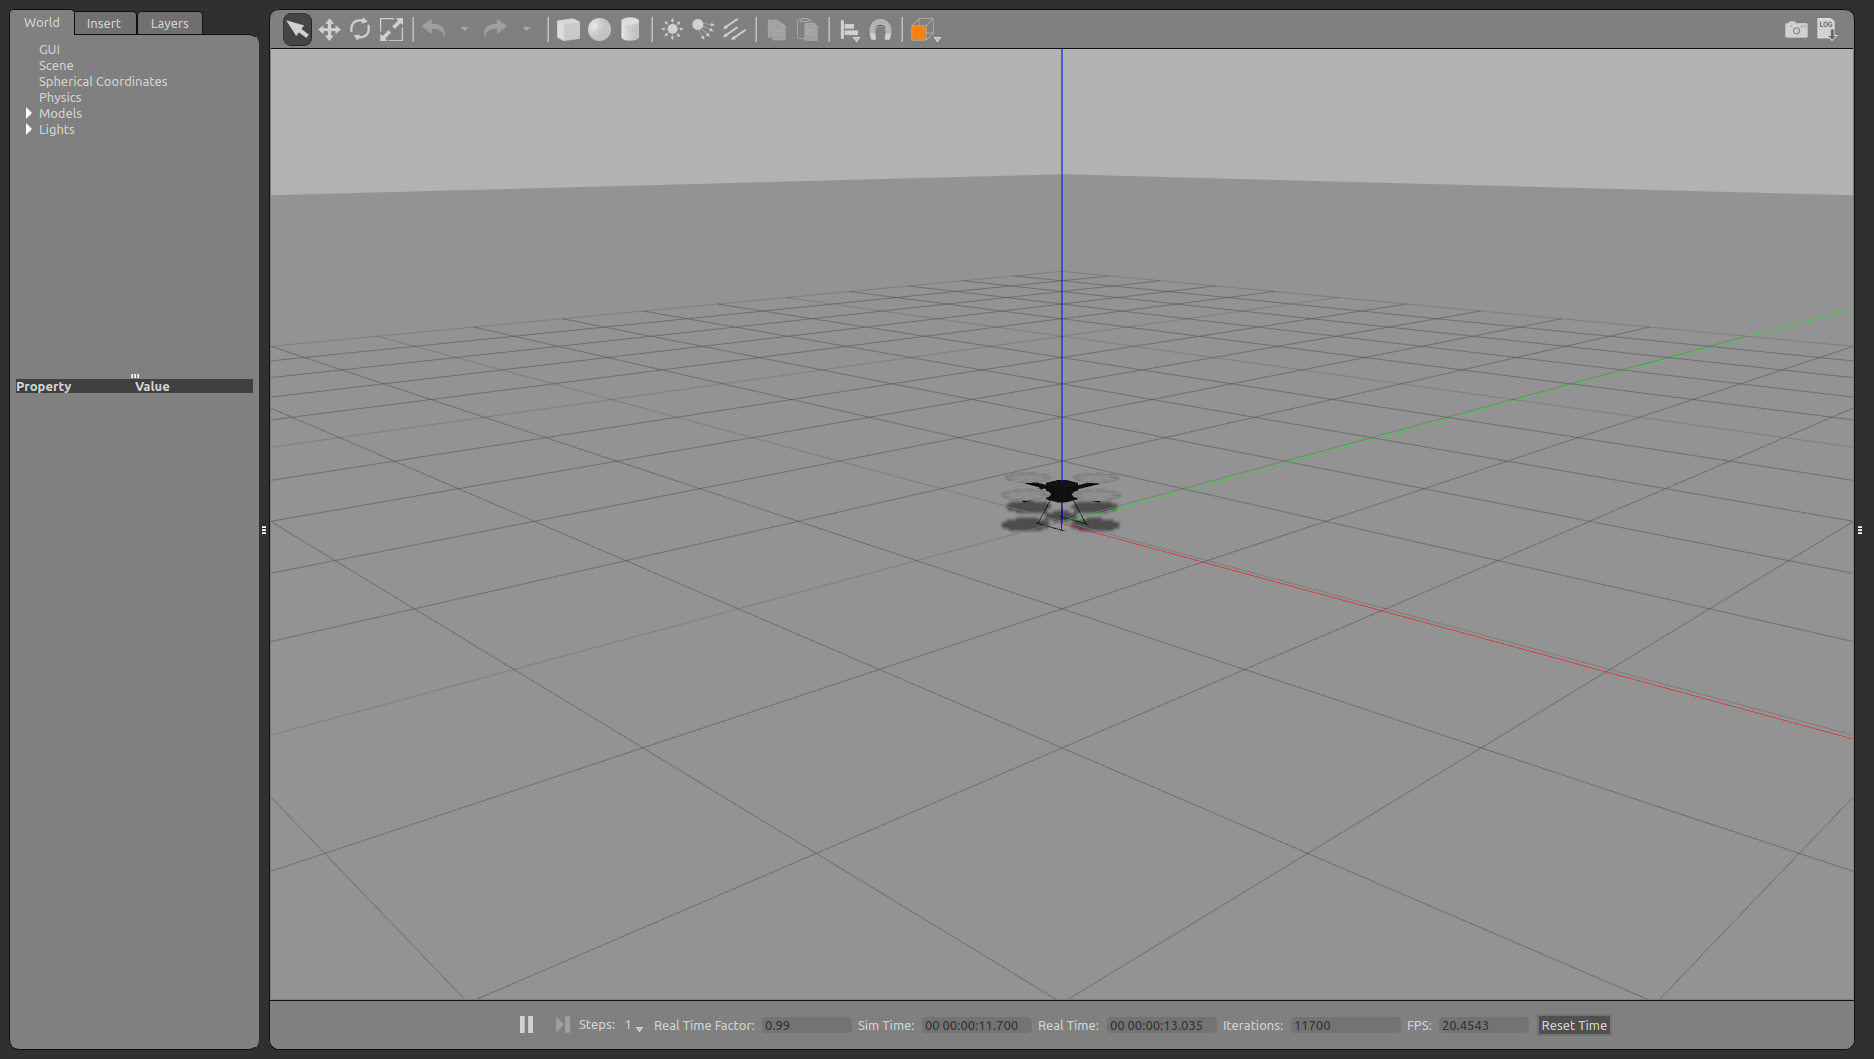
\includegraphics[width=\textwidth]{images/test/drone_gazebo.png}
        \caption{การจำลอง quadrotor ด้วยโปรแกรม Gazebo}
    \end{subfigure}
    \hfill
    \begin{subfigure}[b]{0.8\textwidth}
        \centering
        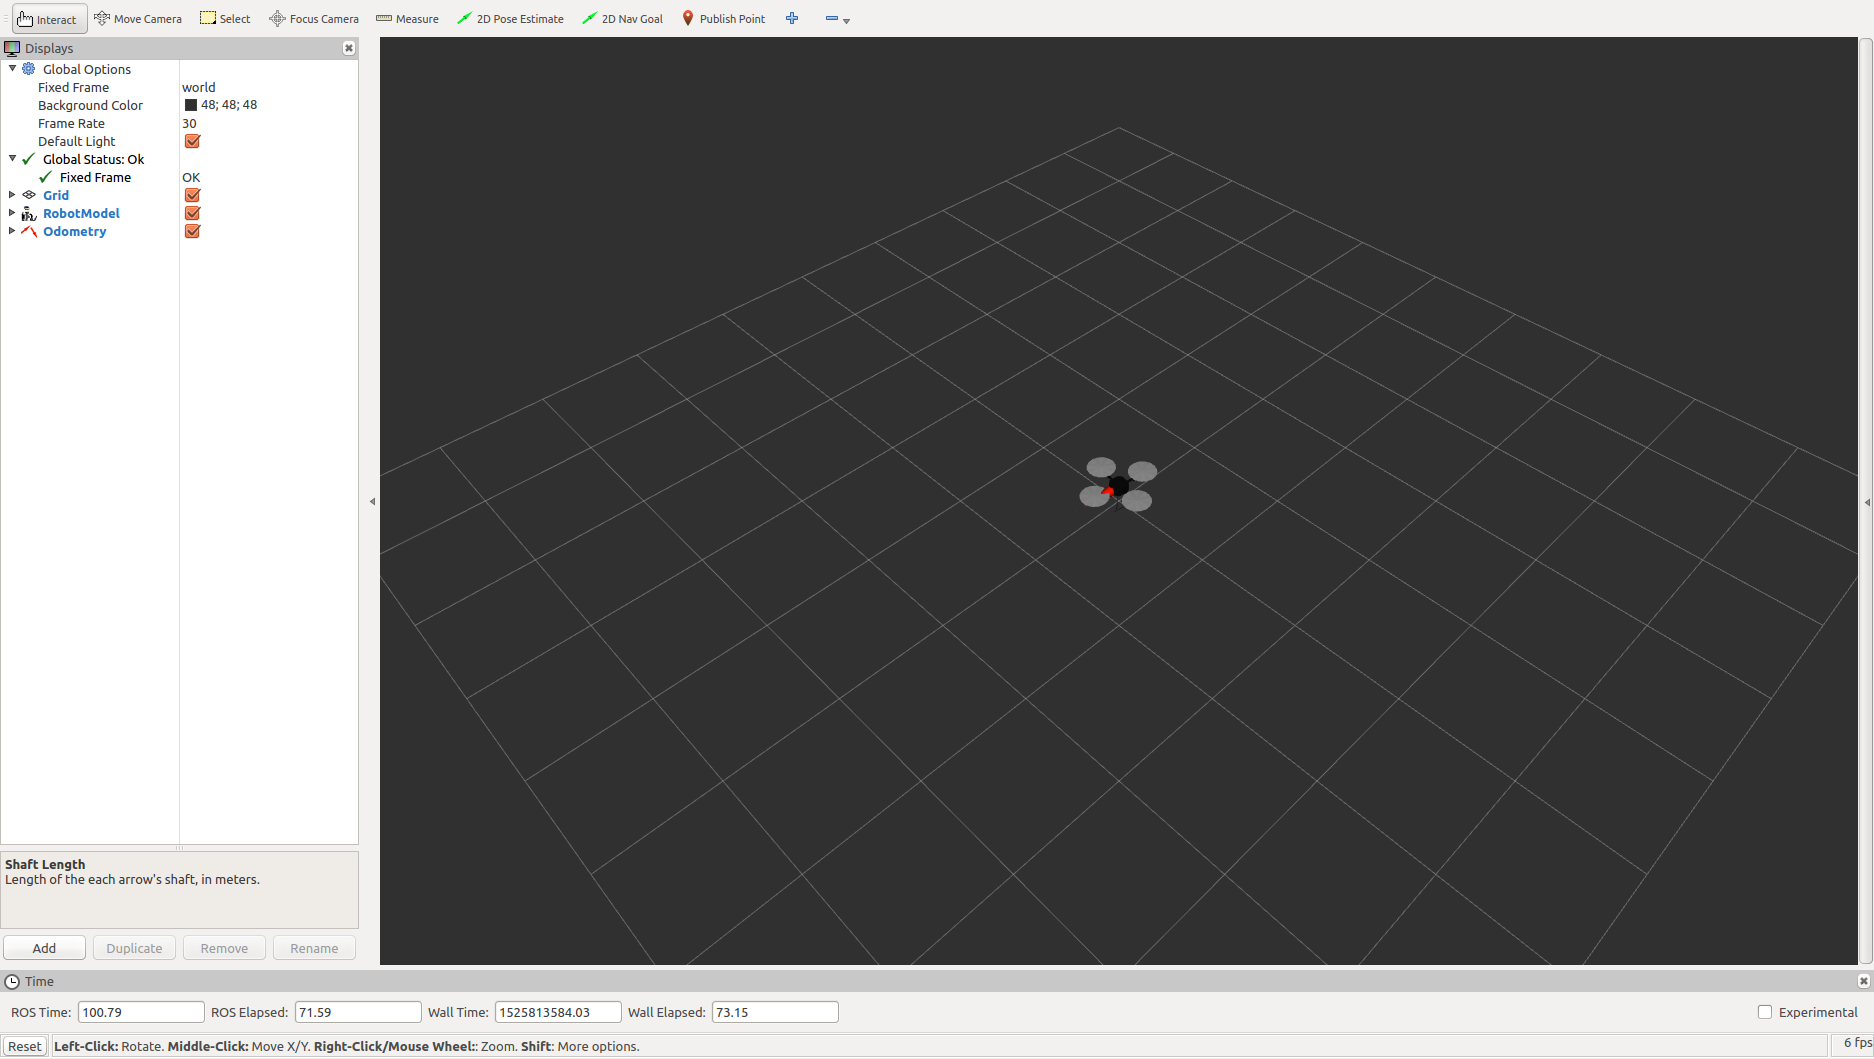
\includegraphics[width=\textwidth]{images/test/drone_rviz.png}
        \caption{การแสดงผลภาพ quadrotor ด้วยโปรแกรม Rviz}
    \end{subfigure}
    \caption{การจำลองและการแสดงผลภาพของ quadrotor }
\end{figure}

\clearpage
\subsection{สั่งให้ quadrotor บินขึ้นเหนือพื้น}
\begin{figure}[!ht]
	\centering
	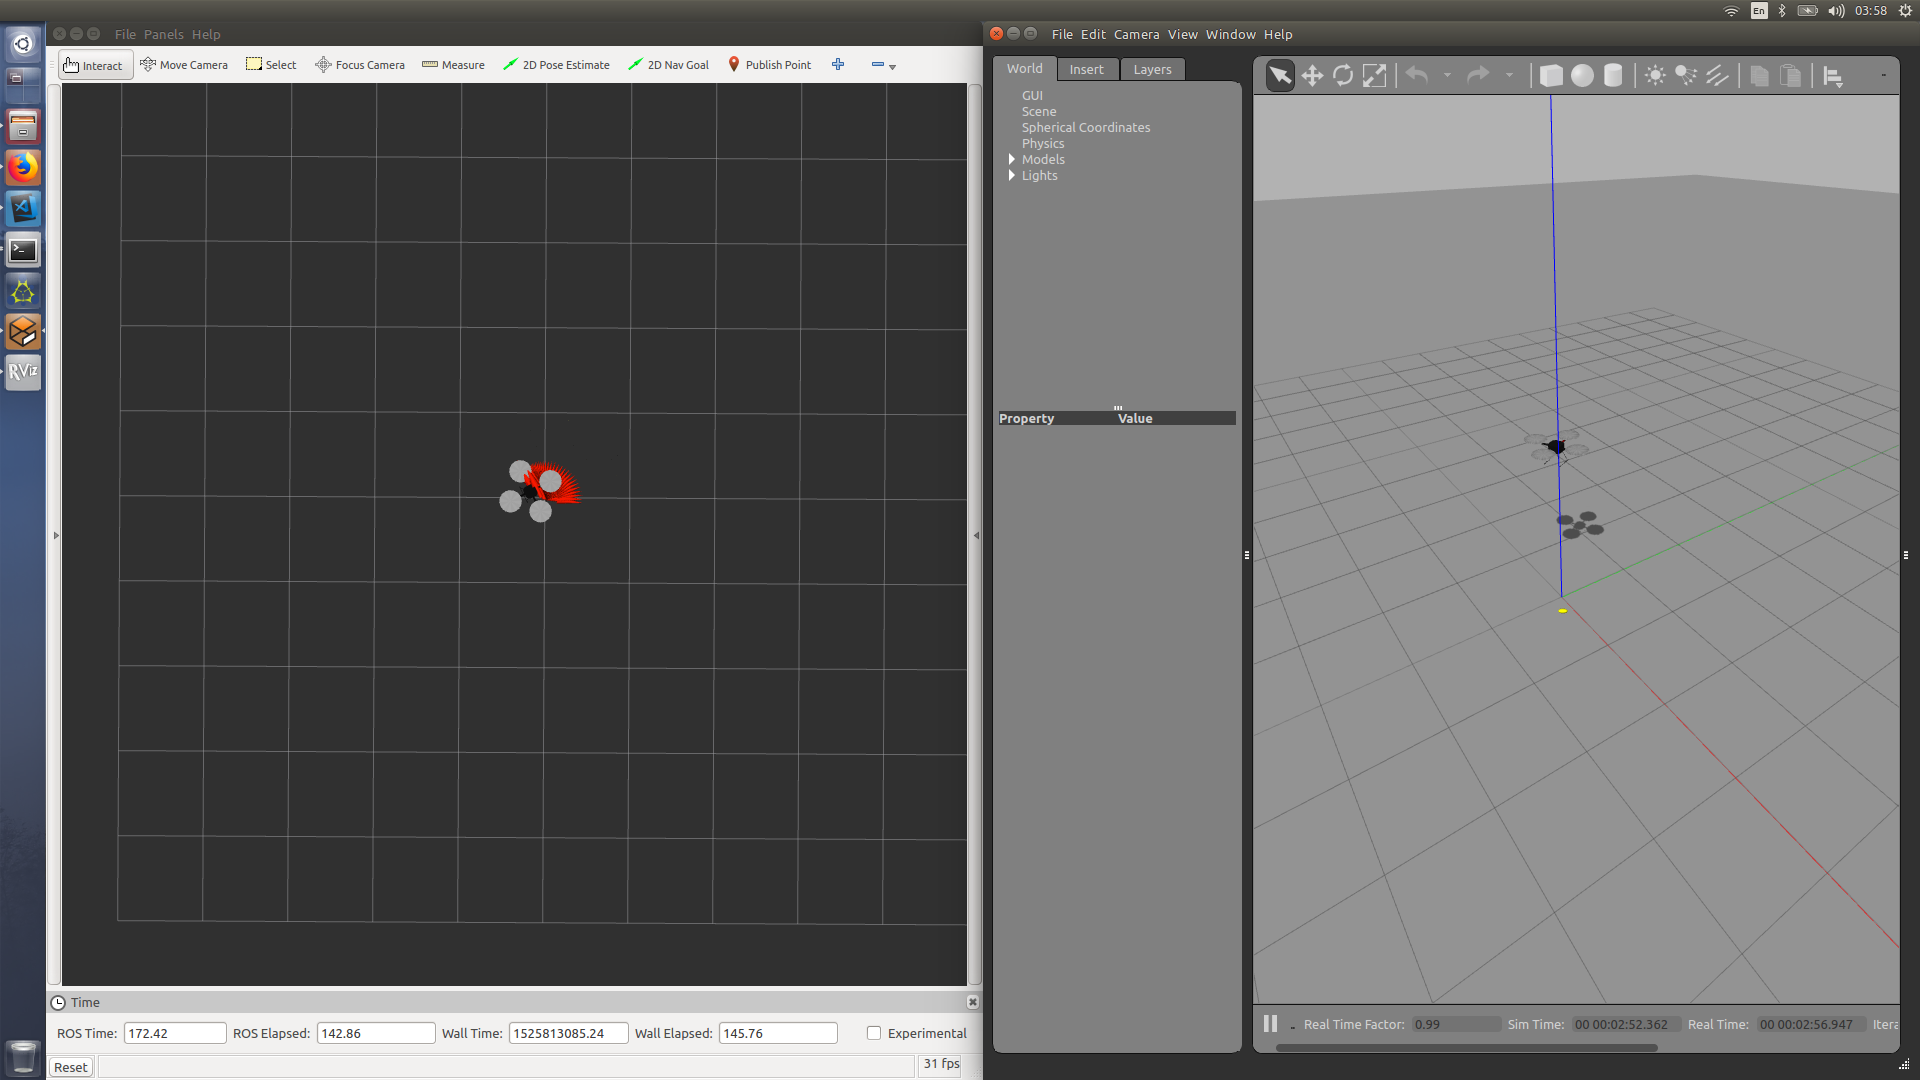
\includegraphics[width=0.7\textwidth]{images/test/drone_takeoff.png}
	\caption{ผลการสั่งให้ quadrotor บินขึ้นเหนือพื้น 2 เมตร}
\end{figure}

\subsection{สั่งให้ quadrotor บินวนเป็นเกลียว}
\begin{figure}[!ht]
    \centering
    \begin{subfigure}[b]{0.67\textwidth}
        \centering
        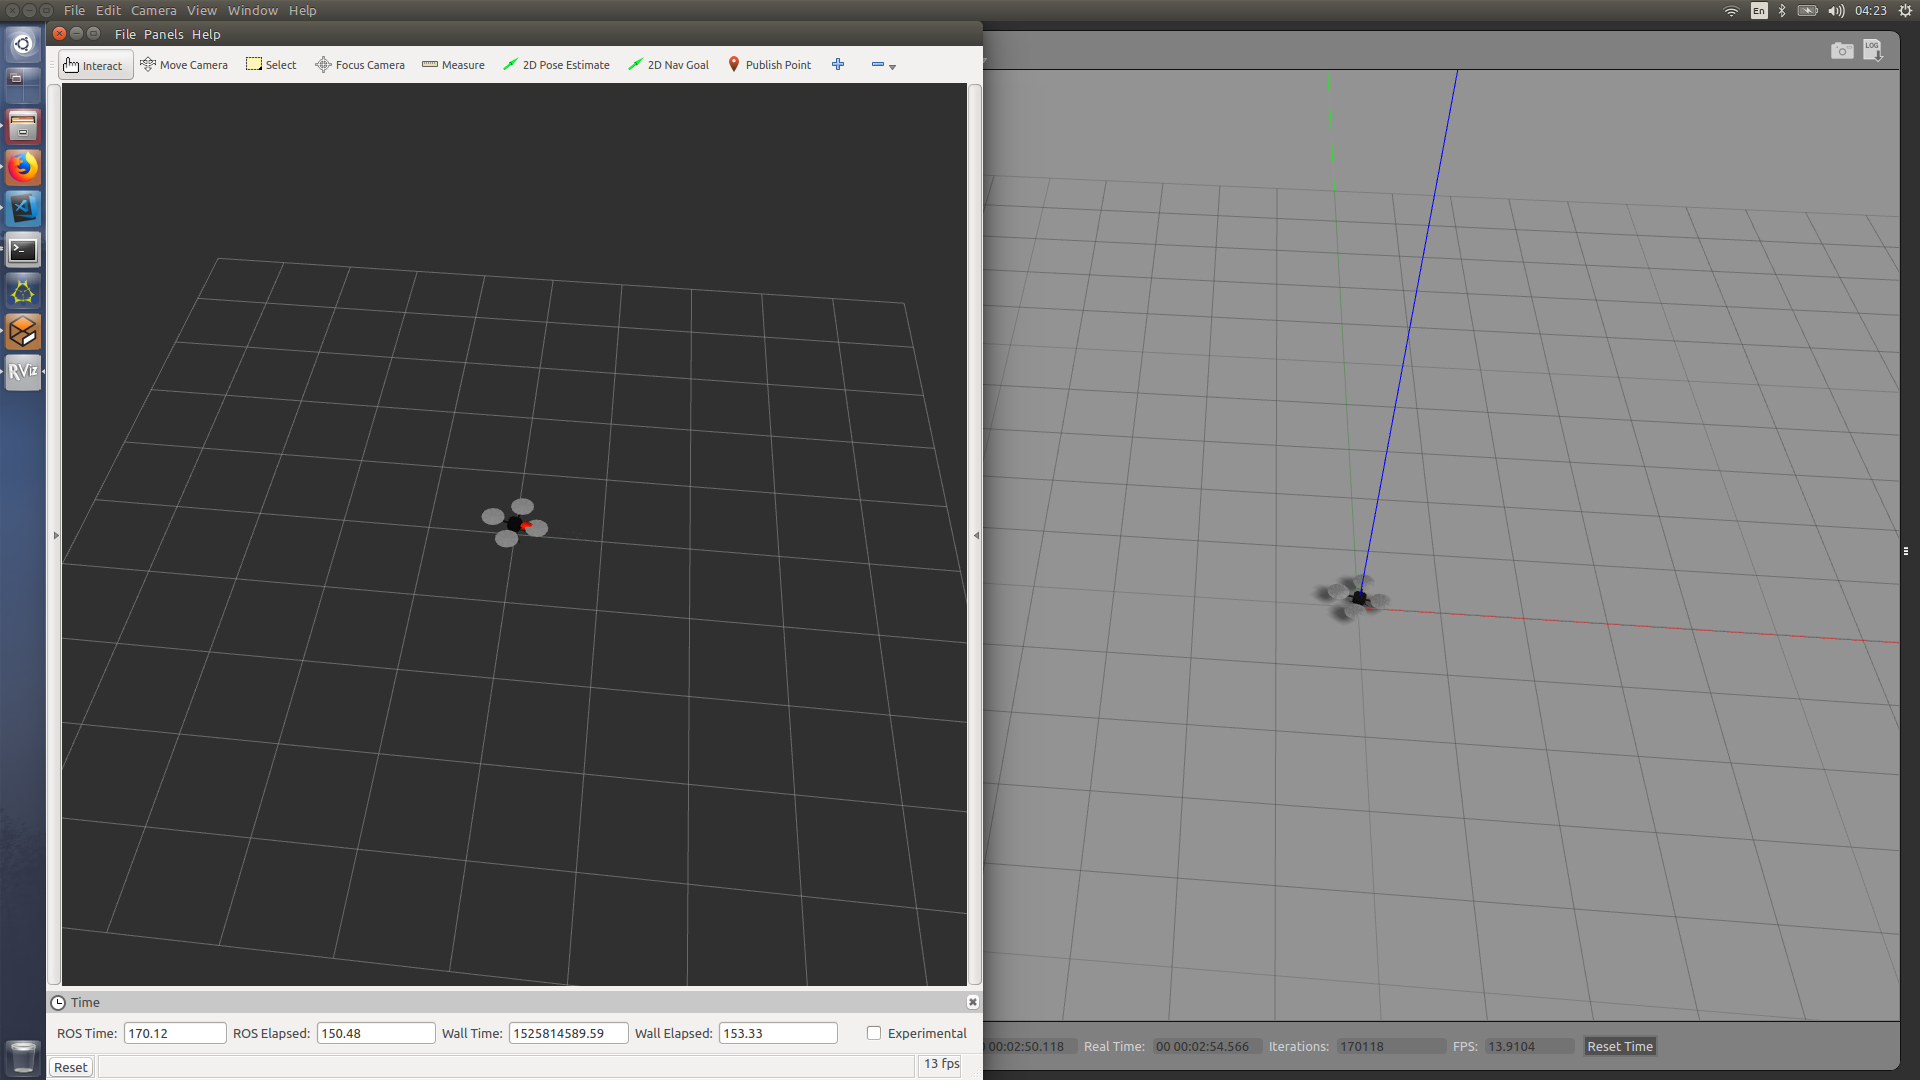
\includegraphics[width=\textwidth]{images/test/circle1.png}
        \caption{quadrotor บินวนเป็นเกลียว ขั้นที่ 1}
    \end{subfigure}
    \hfill
    \begin{subfigure}[b]{0.67\textwidth}
        \centering
        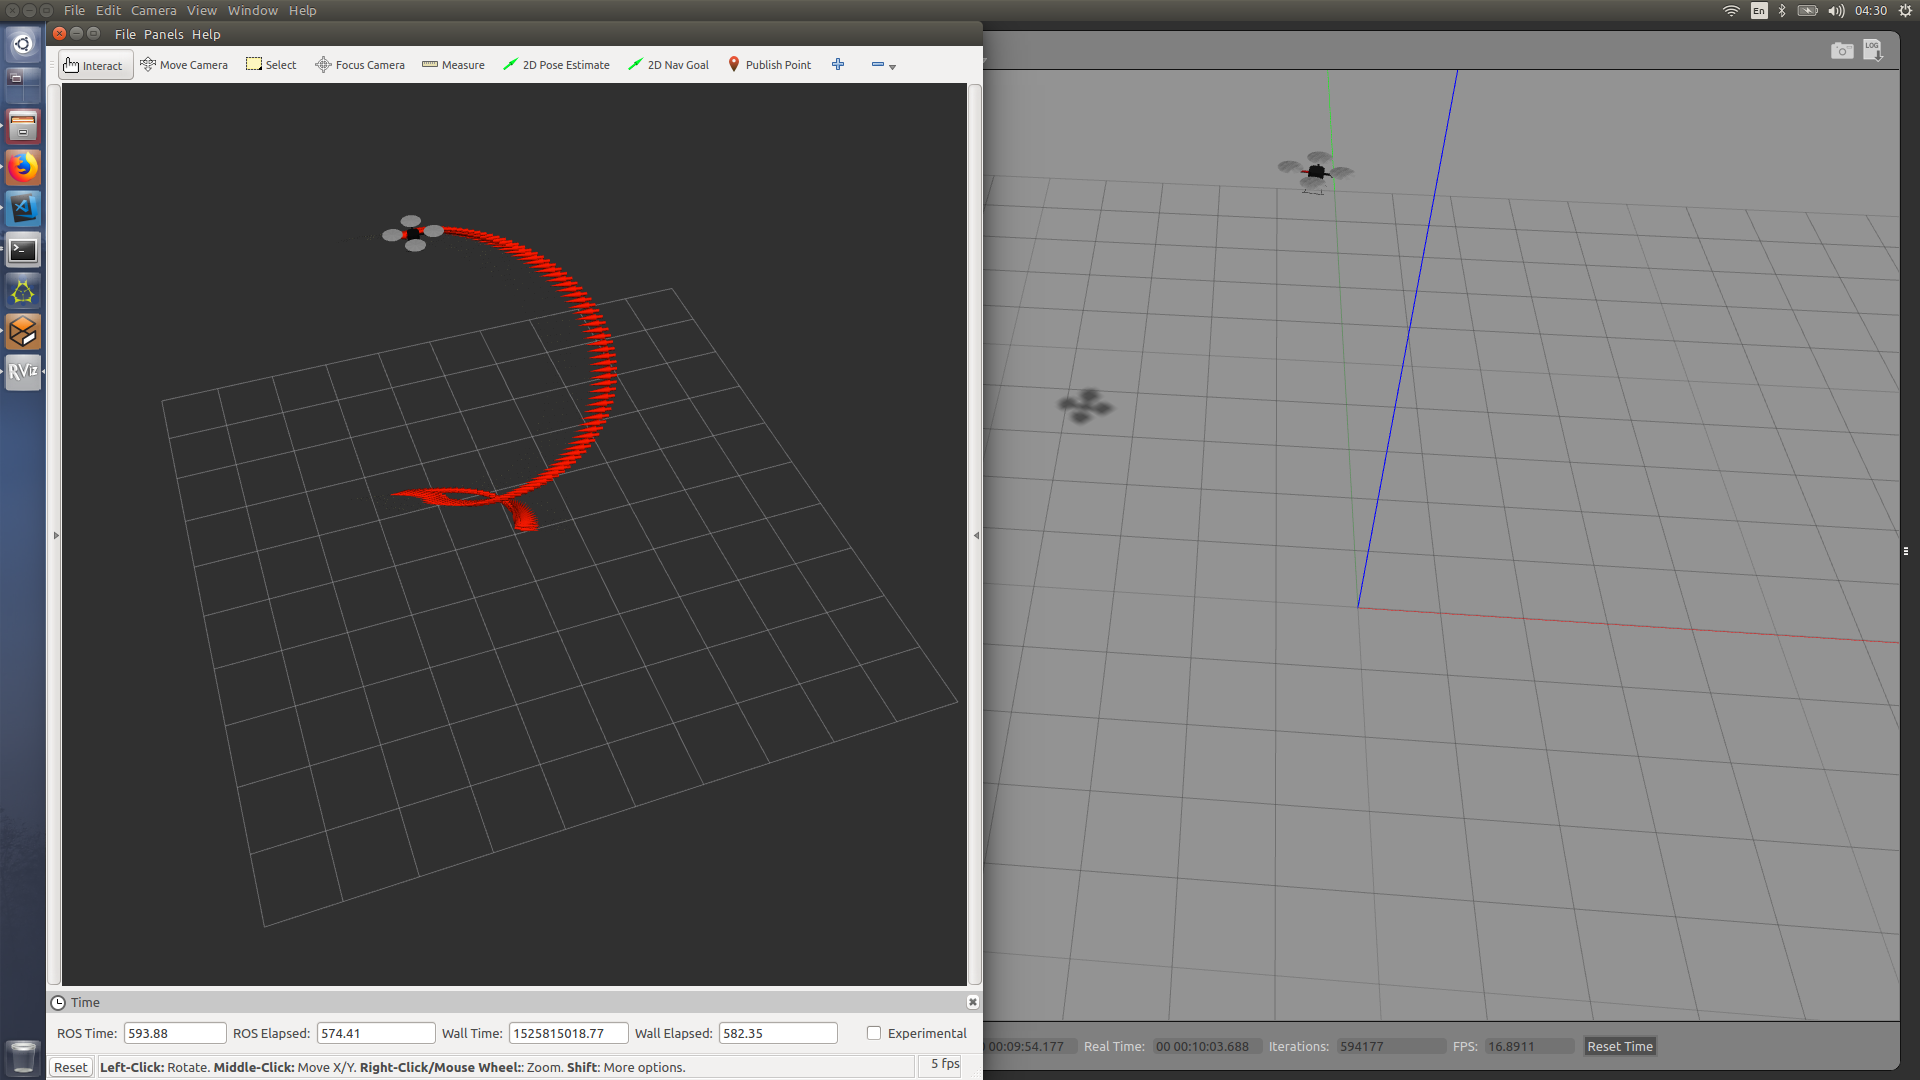
\includegraphics[width=\textwidth]{images/test/circle2.png}
        \caption{quadrotor บินวนเป็นเกลียว ขั้นที่ 2}
    \end{subfigure}
    \caption{ผลการสั่งให้ quadrotor บินวนเป็นเกลียว}
\end{figure}

\clearpage
\subsection{สั่งให้ quadrotor บินเป็นรูปดาว}
\begin{figure}[!ht]
    \centering
    \begin{subfigure}[b]{0.7\textwidth}
        \centering
        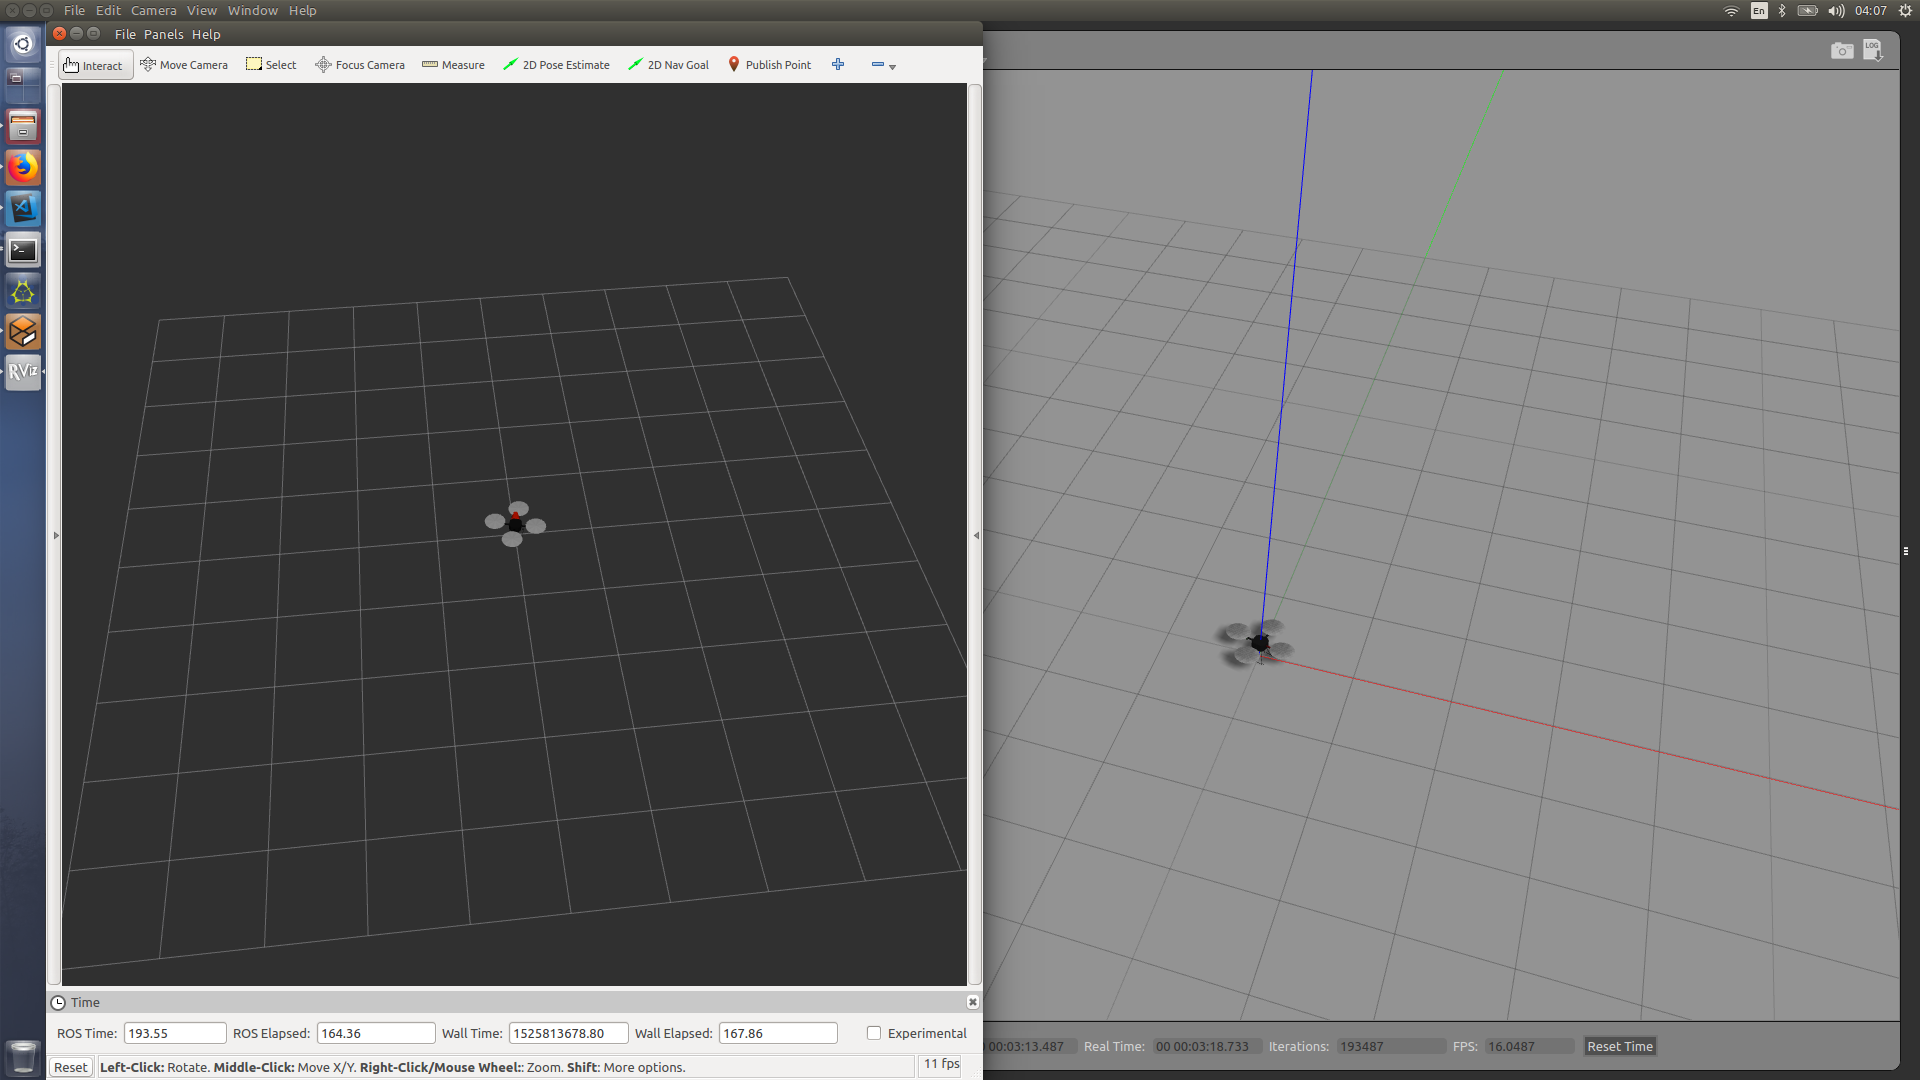
\includegraphics[width=\textwidth]{images/test/drone_rg1.png}
        \caption{quadrotor บินเป็นรูปดาว ขั้นที่ 1}
	\end{subfigure}
	\hfill
    \begin{subfigure}[b]{0.7\textwidth}
        \centering
        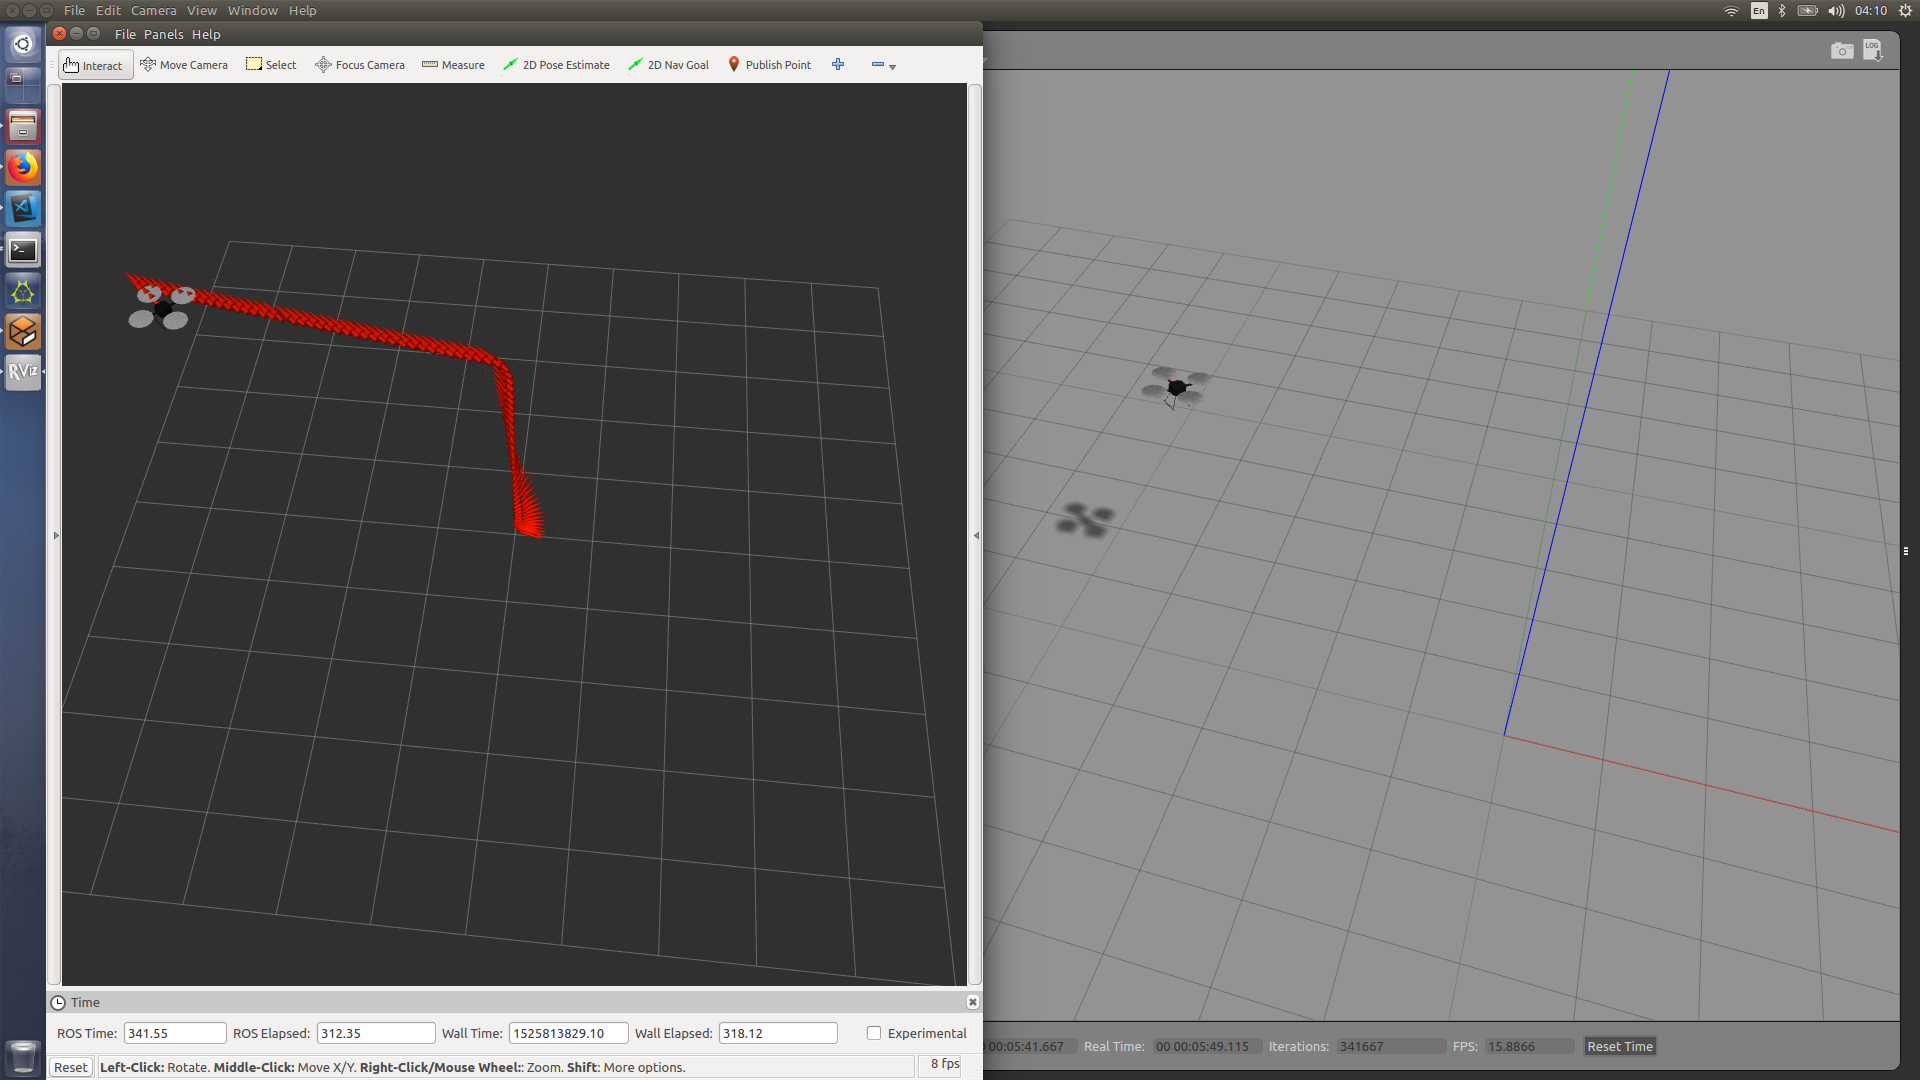
\includegraphics[width=\textwidth]{images/test/drone_rg2.png}
        \caption{quadrotor บินเป็นรูปดาว ขั้นที่ 2}
    \end{subfigure}
    \hfill
    \begin{subfigure}[b]{0.7\textwidth}
        \centering
        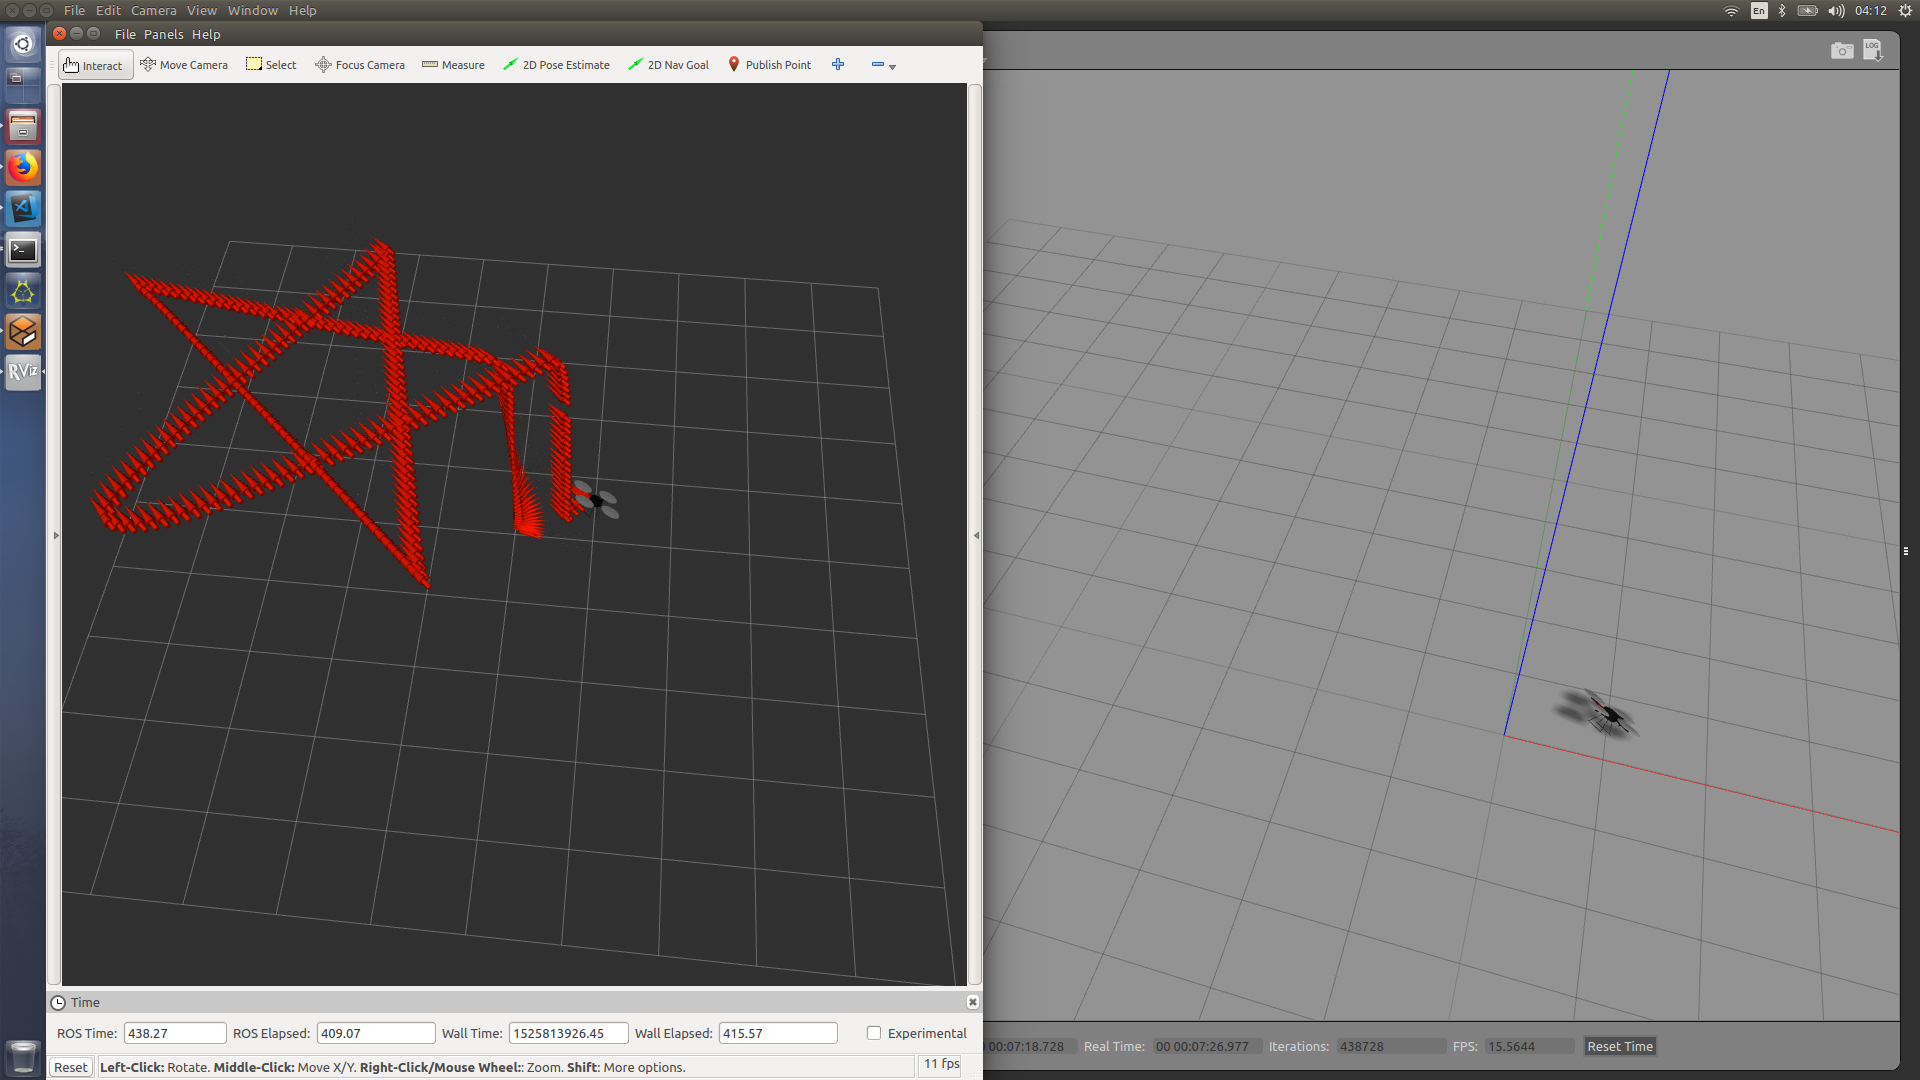
\includegraphics[width=\textwidth]{images/test/drone_rg3.png}
        \caption{quadrotor บินเป็นรูปดาว ขั้นที่ 3}
    \end{subfigure}
    \caption{ผลการสั่งให้ quadrotor บินเป็นรูปดาว}
\end{figure}